\documentclass[]{tp}
\titre{TP15 : Ondes ultrasonores}  
\begin{document}
%\small

\section{Création et réception d'une onde sonore}
Le but de cette partie est de générer une onde ultra-sonore à l'aide d'un module émetteur. Puis de visualiser l'onde reçue par un récepteur sur un oscilloscope.
  \begin{center}
  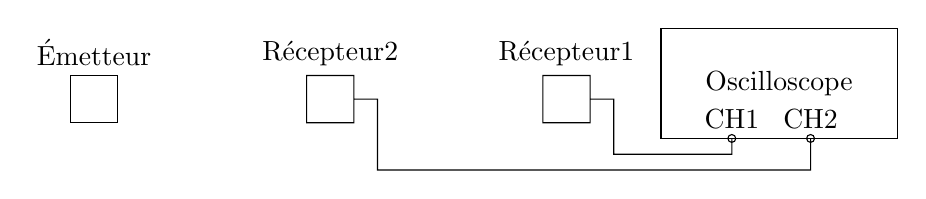
\begin{tikzpicture}[scale=1, transform shape]
    \draw (0,0.3) rectangle ++(0.6,-0.6) ++(-0.3, 0.6) node[above] {Émetteur};
    \draw (0,0) ++(6,0) ++(0,0.3) rectangle ++(0.6,-0.6) ++(-0.3,0.6) node[above]{Récepteur1} ++(0.3, -0.3) -- ++(0.3,0) -- ++(0, -0.7) -- ++(1.5, 0) -- ++(0, 0.2) circle (0.05) node[above]{CH1} ;
    \draw (0,0) ++(3,0) ++(0,0.3) rectangle ++(0.6,-0.6) ++(-0.3,0.6) node[above]{Récepteur2} ++(0.3, -0.3) -- ++(0.3,0) -- ++(0, -0.9) -- ++(5.5, 0) -- ++(0, 0.4) circle (0.05) node[above]{CH2} ;
    \draw (0,0) ++(9,0.2) node[rectangle, draw, minimum width=3cm, minimum height=1.4cm]{Oscilloscope};
  \end{tikzpicture}
  \end{center}
  
\subsection{Réglages préliminaires}
Le module émetteur d'ultrasons contient un oscillateur qui alimente l'émetteur avec une fréquence autour de \SI{40}{\kilo\hertz}. 

Les transducteurs ultrasonores ont une fréquence de fonctionnement optimale, c'est à dire qu'il existe une fréquence pour laquelle l'amplitude qu'ils émettent est maximale.

On commence donc par ajuster la fréquence de l'émetteur pour que le signal reçu soit maximum.

Les récepteurs sont branchés directement sur l'entrée de l'oscilloscope. On règlera le déclenchement de l'oscilloscope sur le récepteur 1 qui restera fixe.

\section{Mesure des caractéristiques de l'onde}
On souhaite maintenant mesurer les paramètres qui caractérisent l'onde ultrasonore émise. On s'intéresse notamment à sa fréquence, sa longueur d'onde et sa célérité.
\begin{itemize}
  \item Comment changent les signaux observés sur l'oscilloscope lorsqu'on éloigne le récepteur 2 de l'émetteur ? Expliquer ce phénomène.

  \item Pour mesurer la longueur d'onde de l'onde émise, on commence par disposer l'émetteurs et les récepteurs face à face le long d'un réglet gradué. On les place assez proches l'un de l'autre et de telle manière que les signaux observés à l'oscilloscope soient en phase. Puis on éloigne le récepteur 2, lorsqu'on l'a éloigné d'une longueur d'onde, les signaux sont à nouveau en phase.

    Mesurer de cette manière la longueur d'onde de l'onde émise en essayant de l'optimiser pour obtenir la mesure la plus précise possible 
    \begin{itemize}
      \item On pourra par exemple mesurer la distance correspondant à plusieurs longueurs d'onde
      \item Pour détecter une différence de phase nulle entre les deux signaux on utilisera le mode \texttt{xy} de l'oscilloscope (Comment ?)
    \end{itemize}

  \item Déduire de vos mesures de longueur d'onde et de fréquence une estimation de la célérité de l'onde ainsi que l'incertitude associée. On peut obtenir une valeur de la vitesse du son dans l'air à la température $T$ (en degrés celsius entre -20 et \SI{+40}{\celsius}) avec une erreur inférieure à \SI{0.2}{\percent} avec la formule approchée :
    \begin{equation*}
      c=(331.5+0.607\cdot T)~\si{\m\per\s}
    \end{equation*}
    La valeur calculée est-elle compatible avec celle que vous avez mesurée ?

  \item L'émetteur peut être réglé pour envoyer des impulsions ultrasonores. Utiliser cette fonctionnalité pour faire une mesure directe de la vitesse du son dans l'air. Comparer la mesure obtenue à la valeur précédente.
\end{itemize}

\section{Interférences}%
\label{sec:interferences}

On souhaite maintenant observer des interférences entre ondes ultrasonores. On pourrait imaginer utiliser deux émetteurs différents et mesurer la superposition des ondes émises mais cette méthode risque fort de ne pas fonctionner. Pourquoi ?

En utilisant un seul émetteur, on peut mettre en place un écran pour qu'une partie des ondes émises pas l'émetteur atteignent directement le récepteur alors qu'une autre partie se réfléchit sur l'écran avant d'atteindre le récepteur.

Nous allons mettre en place une expérience utilisant le principe décrit ci-dessus en essayant au maximum de se rapprocher de la configuration ``trous d'Young" et mesurer la figure d'interférences. 

On pourra effectuer un montage similaire à celui présenté sur la figure ci-dessous

\begin{center}
  \begin{tikzpicture}
    \draw[rotate = 40, yshift=-1cm] (0, 0) rectangle ++(0.6,0.6) ++ (-0.3, 0) node[above, rotate=40]{émetteur} ++( 0.3, -0.3) coordinate (A);
    \draw[thick] (0,2) -- ++(3, 0) ++(-1.5, 0) node[above]{écran};
    \draw[-latex] (10, -2) -- (10, 2) node[right]{$x$};
    \draw (10, 0.5) rectangle ++(0.6, 0.6) ++(0, -0.3) node[right]{récepteur};
    \draw[rayon] (A) -- (1.5, 2);
    \draw[rayon] (1.5,2) -- (10, 0.8) coordinate(B);
    \draw[rayon] (A) -- (B);
  \end{tikzpicture}
\end{center}

\begin{itemize}
  \item Enregistrer l'amplitude reçue $A(x)$ en fonction de $x$ en positionnant l'écran et l'émetteur pour observer les interférences les plus contrastées possibles. 

  \item Comparer l'évolution de $A(x)$ à celle que l'on obtiendrait dans une configuration de ``trous d'Young" idéale. 
\end{itemize}
\end{document}
